\documentclass[french]{msereport}

\usepackage{minted}
\usepackage{tabularx}

\newcommand{\gae}{\brand{Google App Engine}}

\title{Platform as a Service : \gae}
\module{CLOUD}{Cloud Computing}
\author{Jonathan Cornaz}

\begin{document}
	
	\section{Introduction}
		Dans le but d'appréhender le développement et le déploiement d'application dans un \eng{cloud} de type "platform as a service", deux \eng{servlets} ont été créés et déployés sur \gae. Une fois déployé, des tests de performances ont été effectués afin d'observer les mécanismes d'\eng{auto-scaling} de la plateforme.

	\subtitledsection[Exercice 1]{Déploiement d'une simple application web}
		L'exemple généré est un simple "Hello world". Il est constitué de trois fichiers clés : \code{index.html}, \code{web.xml} et \code{Lab04Servlet.java}.
		
		\subsection{Fichier index.html}
			A la racine de l'application apparaît un fichier \code{index.html} qui contient une redirection vers l'url "/Labo04".
		
		\subsection{Fichier web.xml}
			Le fichier de description d'application web (\code{web.xml}) définit le fichier par défaut à utiliser si l'url ne contient pas de chemin spécifique (en l'occurence \code{index.hml}). Et il contient également le mappage de l'url "/Labo4" avec l'applet java \code{ch.hesso.mse.cloud.cornaz.Lab04Servlet}.
		
		\subsection{Fichier *.java}
			Le servlet (\code{Lab04Servlet.java}) est une classe dérivée de \code{HttpServlet} qui implémente une méthode {doGet(HttpServletRequest, HttpServletResponse)}. En l'occurence l'implémentation consiste en la déclaration d'un contenu texte et de l'impression du message "Hello world".
			
			
	\subtitledsection[Exercice 2]{Développer un \eng{Servlet} qui utilise le magasin de donnée}
		Pour créer un \eng{servlet} qui utilise le magasin de donnée, il a suffit d'écrire la classe suivante :
		\inputminted[
				frame=lines,
				fontsize=\footnotesize,
				linenos,
				label=ch.hesso.mse.cloud.cornaz.DatastoreWrite,
				firstline=17
			]
			{java}
			{../Lab04/src/ch/hesso/mse/cloud/cornaz/DatastoreWrite.java}
		
		\clearpage
		Une fois la classe dévloppé elle a été \eng{mappée} dans le fichier \code{web.xml} :
				\inputminted[
				frame=lines,
				fontsize=\footnotesize,
				linenos,
				label=web.xml,
				]
				{xml}
				{../Lab04/war/WEB-INF/web.xml}
				
		\clearpage
		Après quelques essais, en local et sur la version déployée dans le \eng{cloud}, les magasins de données avaient la teneur suivante :
		
		\begin{figure}[h]
			\label{ds_viewer_local}
			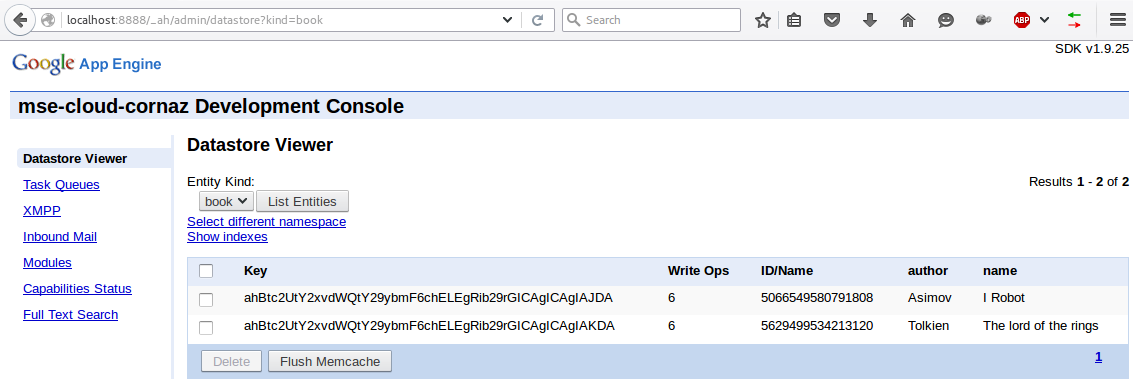
\includegraphics[width=\textwidth]{screen_ds_viewer_local.png}
			\caption{Résultat dans le magasin de donnée en local}
		\end{figure}
				
		\begin{figure}[h]
			\label{ds_viewer_cloud}
			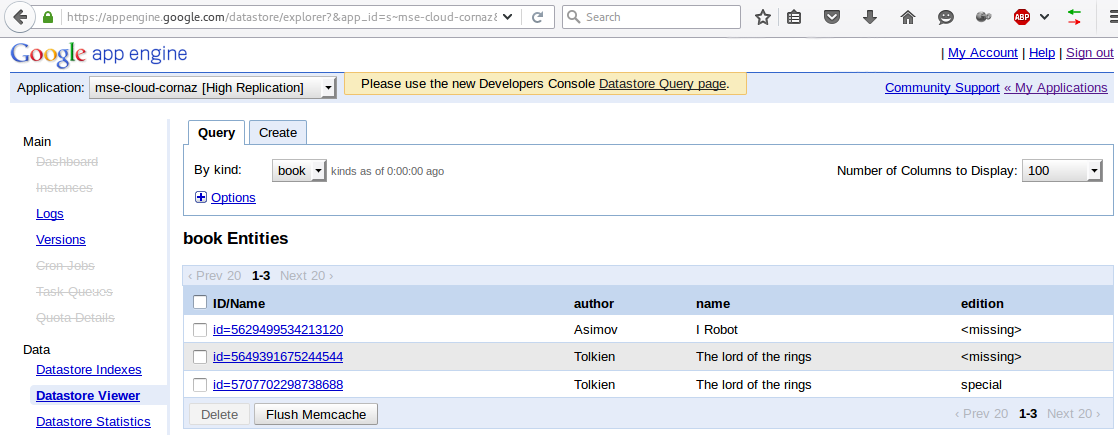
\includegraphics[width=\textwidth]{screen_ds_viewer_cloud.png}
			\caption{Résultat dans le magasin de donnée du \eng{cloud}}
		\end{figure}
		
	
	\subtitledsection[Exercice 3]{Tester les performances d'écriture du magasin de donnée}
		Après avoir déployé l'application, il était question d'évaluer les performances des requêtes et comparer la différence entre les \eng{servlets} \code{DatastoreWrite} et \code{HelloWorld}. Pour ce faire \brand{JMeter} a été utilisé et a simulé pour les deux 5'000 requêtes en une minute.
		
		\subsection{Graphiques}
			Lors de l'execution des tests avec \brand{JMeter}, les temps de réponses ont évolués de la manière suivante :
			
			\begin{figure}[!h]
				\label{perf_dswrite}
				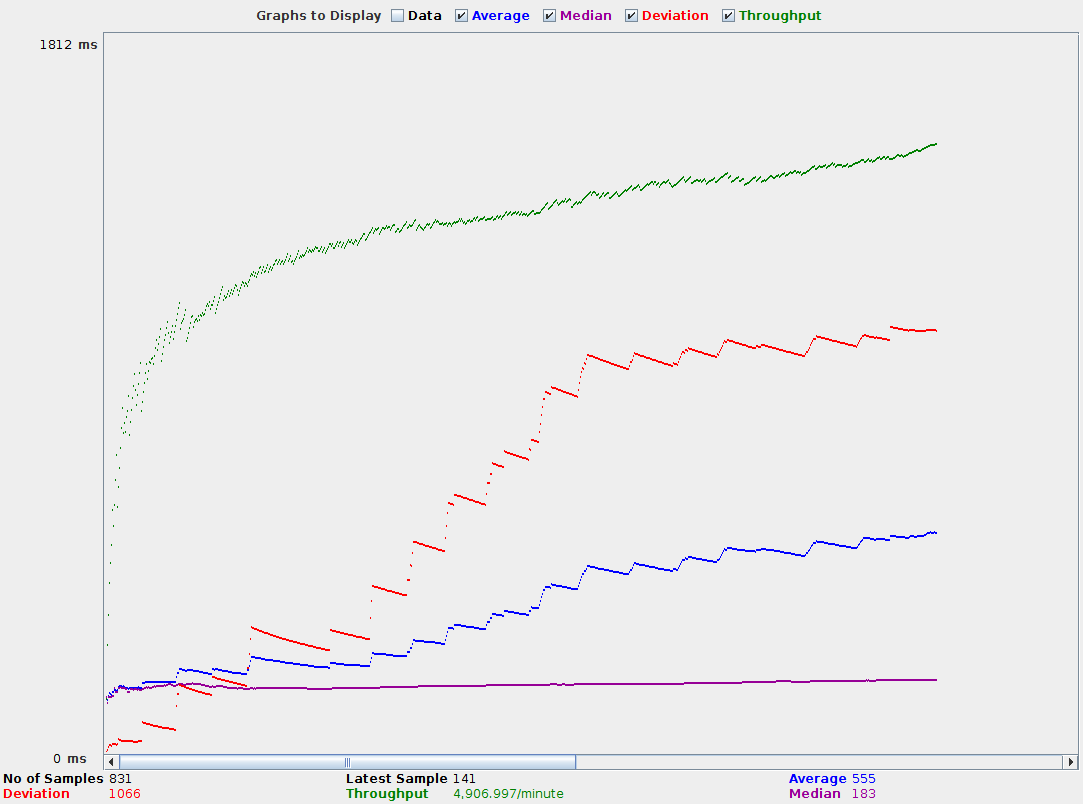
\includegraphics[width=\textwidth]{screen_jmetter_dswrite.png}
				\caption{Temps de réponse de requête impliquant des écritures dans le magasin de donnée}
			\end{figure}
			
			On constate qu'il y a des sortes d'à-coups. Après la création d'une instance, le temps de réponse décroit progressivment, jusqu'à (semble-t-il) ce que la quantité de requête à gérée soit à nouveau trop importante et que \gae\ crée automatiquement une nouvelle instance. Ce processus est cyclique, mais on remarque qu'il se stabilise, lorsque le nombre d'instance semble suffisant pour absorber complètement le flux de requêtes.
			
			\clearpage
			\begin{figure}[!h]
				\label{perf_helloworld}
				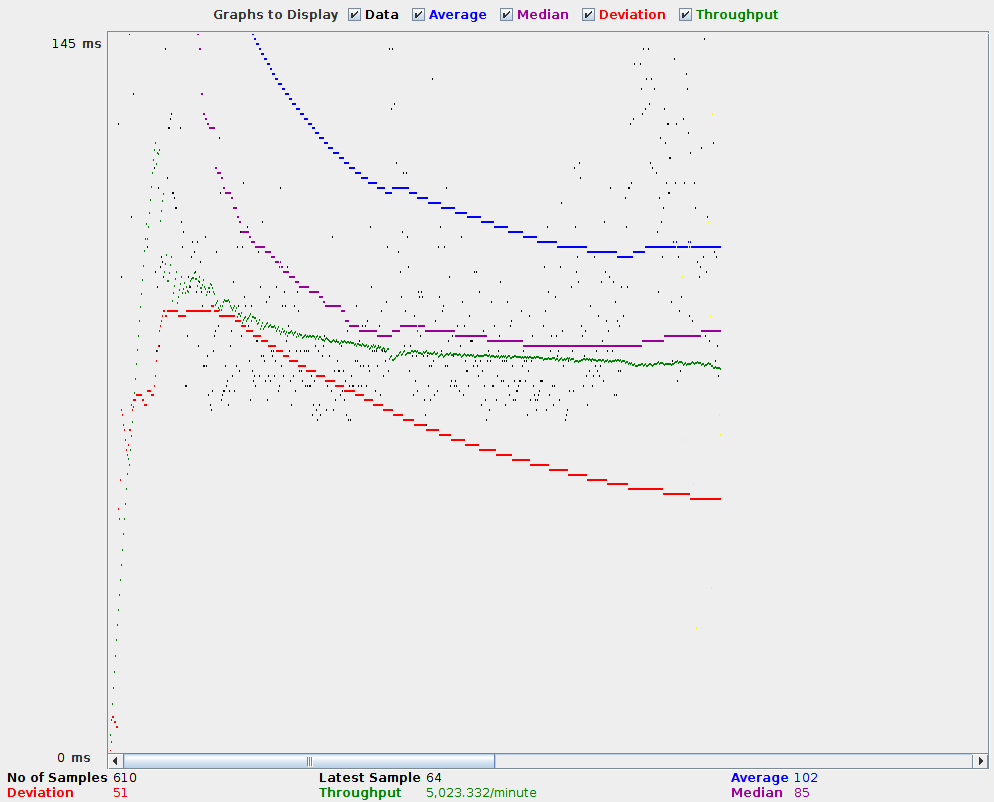
\includegraphics[width=\textwidth]{screen_jmeter_helloworld.png}
				\caption{Temps de réponse de requête sans implication du magasin de donnée}
			\end{figure}
			
			
			Le service "Hello world" réagit de même, mais pendant beaucoup moins longtemps. Après les deux premières instances créées par \gae, il est capable d'absorber les requêtes et d'y répondre en une centaine de millisecondes. La plateforme n'a donc pas besoin de créer plus d'instances.

				
		\subsection{Temps de réponses}
			Les temps de réponses du \eng{servlet} qui utilise le magasin de donnée sont en moyenne de l'ordre de la demi seconde. Alors que les temps de réponses du \eng{servlet} "Hello world" qui n'utilise pas le magasin de donnée, les temps de réponses sont presque tous en dessous des deux dixièmes de secondes.
			
			Cela s'explique par le fait que les opérations en écriture on un coup en temps bien plus élevé puisqu'il faut faire intervenir le magasin de donnée et attendre que la transaction ait été complètement sauvegardée de manière cohérente et pérenne. Alors que le "Hello world", quant à lui, n'accède pas du tout au magasin de donnée, même en lecture. Il se contente d'afficher un message prédéfinit. Cette action peut être accomplie de manière beaucoup plus rapide, puisque le seul "frein" est simplement la rapidité de traitement de la requête.
		
		\clearpage
		\subsection{Quotas utilisés}
			
			Le quota le plus utilisé est celui des opérations d'écriture dans le magasin de donnée. Celui-ci ne permet que 50'000 opérations en écriture. Comme les test effectuaient chaque fois 5'000 enregistrement, il n'a suffit que de quelqu'uns d'entre eux pour remplir le quotas.
			
			\begin{table}[!h]
				\setlength\extrarowheight{3pt}
				\caption{Quotas quotidiens utilisés}
				\label{tab:quotas}
				\begin{tabularx}{\textwidth}{|l|r|X|}
					\hline
					\textbf{Quota}			& \textbf{Utilisé}	& \textbf{Explication} \\
					\hline
					Bande passante sortante				& 1\%	& Car les deux \eng{servlets} ne retourne que de simple messages plein-textes \\
					\hline
					Bande passante entrante 			& 0\%	& Les requêtes étaient simples et n'on jamais envoyée de donnée lourde \\
					\hline
					Heures d'instances frontend			& 3\%	& Même s'il y a eu beaucoup d'instances, les tests n'ont durés que quelques minutes \\
					\hline
					Écriture dans le \eng{datastore}	& 94\%	& Comme expliqué c'est l'aspect principal dont les performances ont été testées \\
					\hline
					Lecture dans le \eng{datastore}		& 0\%	& Mis à part un ou deux tests manuels, il n'y a eu aucune lecture des données \\
					\hline
				\end{tabularx}
			\end{table}
			
			\begin{figure}[!h]
				\label{quotas}
				\centering
				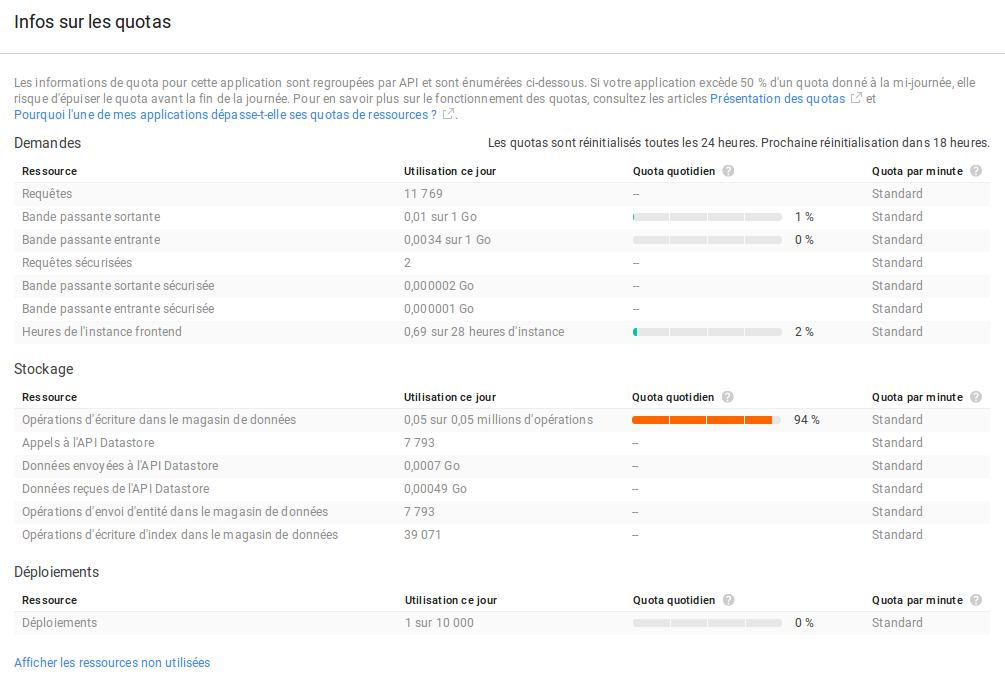
\includegraphics[width=\textwidth]{screen_quotas.png}
				\caption{Quotas utilisés}
			\end{figure}
			
		\clearpage
		\subsection{Suppositions de fonctionnement de \gae}
			Bien que \brand{Google} ne donne pas beaucoup de détails quant au fonctionnement de l'\eng{auto-scaling}, on peut supposer qu'il se base (au moins) sur les valeurs suivantes :
			
			\begin{itemize}
				\item Nombre de requête par seconde lors de la dernière minute
				\item Latence moyenne lors de la dernière minute
				\item Nombre d'instance en cours
			\end{itemize}
			
	\section{Conclusion}
		Le développement et le déploiement d'application avec \gae\ est facile à prendre en main. Tout est mis à disposition du développeur pour qu'il puisse se focaliser sur le développement de son application sans avoir à se soucier du maintien de la plateforme sur laquelle sont application doit être hébergée. L'\eng{auto-scaling} peut paraître un peu "mystique", puisque l'on a que très peu la possibilité de le gérer. Mais c'est une fonctionnalité très puissante, et une fois encore décharge le développeur d'avoir à se soucier de cet aspect pour son application.
		
		Cependant la nature de ce service peut potentiellement poser problème si l'application déployée subit une attaque de type "Deny of services". Si, \brand{Google} a pris des mesures pour réduire au maximum l'impact de ce genre d'attaque, les quotas vont tous de même être épuisé très rapidement ce qui peut au final quand même occasionner des coûts supplémentaires au propriétaire de l'application, s'il veut maintenir sa disponibilité pour les utilisateurs.

	\appendixsection
		
		\listoffigures
		
		\listoftables
		
		\subsection{Donnée}
			\url{http://mse-cloud.s3-website-eu-west-1.amazonaws.com/labs/paas.html}
\end{document}
